\documentclass[journal,12pt,twocolumn]{IEEEtran}
%
\usepackage{setspace}
\usepackage{gensymb}
\usepackage{xcolor}
\usepackage{caption}
%\usepackage{subcaption}
%\doublespacing
\singlespacing

%\usepackage{graphicx}
%\usepackage{amssymb}
%\usepackage{relsize}
\usepackage[cmex10]{amsmath}
\usepackage{mathtools}
%\usepackage{amsthm}
%\interdisplaylinepenalty=2500
%\savesymbol{iint}
%\usepackage{txfonts}
%\restoresymbol{TXF}{iint}
%\usepackage{wasysym}
\usepackage{hyperref}
\usepackage{amsthm}
\usepackage{mathrsfs}
\usepackage{txfonts}
\usepackage{stfloats}
\usepackage{cite}
\usepackage{cases}
\usepackage{subfig}
%\usepackage{xtab}
\usepackage{longtable}
\usepackage{multirow}
%\usepackage{algorithm}
%\usepackage{algpseudocode}
%\usepackage{enumerate}
\usepackage{enumitem}
\usepackage{mathtools}
%\usepackage{iithtlc}
%\usepackage[framemethod=tikz]{mdframed}
\usepackage{listings}
\usepackage{polynom, amsmath, amssymb}

%\usepackage{stmaryrd}
\let\vec\mathbf


%\usepackage{wasysym}
%\newcounter{MYtempeqncnt}
\DeclareMathOperator*{\Res}{Res}
%\renewcommand{\baselinestretch}{2}
\renewcommand\thesection{\arabic{section}}
\renewcommand\thesubsection{\thesection.\arabic{subsection}}
\renewcommand\thesubsubsection{\thesubsection.\arabic{subsubsection}}

\renewcommand\thesectiondis{\arabic{section}}
\renewcommand\thesubsectiondis{\thesectiondis.\arabic{subsection}}
\renewcommand\thesubsubsectiondis{\thesubsectiondis.\arabic{subsubsection}}

%\renewcommand{\labelenumi}{\textbf{\theenumi}}
%\renewcommand{\theenumi}{P.\arabic{enumi}}

% correct bad hyphenation here
\hyphenation{op-tical net-works semi-conduc-tor}

\lstset{
language=Python,
frame=single, 
breaklines=true,
columns=fullflexible
}



\begin{document}
%

\theoremstyle{definition}
\newtheorem{theorem}{Theorem}[section]
\newtheorem{problem}{Problem}
\newtheorem{proposition}{Proposition}[section]
\newtheorem{lemma}{Lemma}[section]
\newtheorem{corollary}[theorem]{Corollary}
\newtheorem{example}{Example}[section]
\newtheorem{definition}{Definition}[section]
%\newtheorem{algorithm}{Algorithm}[section]
%\newtheorem{cor}{Corollary}
\newcommand{\BEQA}{\begin{eqnarray}}
\newcommand{\EEQA}{\end{eqnarray}}
\newcommand{\define}{\stackrel{\triangle}{=}}
\newcommand{\myvec}[1]{\ensuremath{\begin{pmatrix}#1\end{pmatrix}}}
\newcommand{\mydet}[1]{\ensuremath{\begin{vmatrix}#1\end{vmatrix}}}
\newcommand{\mymat}[1]{\ensuremath{\begin{bmatrix}#1\end{bmatrix}}}

\bibliographystyle{IEEEtran}
%\bibliographystyle{ieeetr}

\providecommand{\nCr}[2]{\,^{#1}C_{#2}} % nCr
\providecommand{\nPr}[2]{\,^{#1}P_{#2}} % nPr
\providecommand{\mbf}{\mathbf}
\providecommand{\pr}[1]{\ensuremath{\Pr\left(#1\right)}}
\providecommand{\qfunc}[1]{\ensuremath{Q\left(#1\right)}}
\providecommand{\sbrak}[1]{\ensuremath{{}\left[#1\right]}}
\providecommand{\lsbrak}[1]{\ensuremath{{}\left[#1\right.}}
\providecommand{\rsbrak}[1]{\ensuremath{{}\left.#1\right]}}
\providecommand{\brak}[1]{\ensuremath{\left(#1\right)}}
\providecommand{\lbrak}[1]{\ensuremath{\left(#1\right.}}
\providecommand{\rbrak}[1]{\ensuremath{\left.#1\right)}}
\providecommand{\cbrak}[1]{\ensuremath{\left\{#1\right\}}}
\providecommand{\lcbrak}[1]{\ensuremath{\left\{#1\right.}}
\providecommand{\rcbrak}[1]{\ensuremath{\left.#1\right\}}}
\theoremstyle{remark}
\newtheorem{rem}{Remark}
\newcommand{\sgn}{\mathop{\mathrm{sgn}}}
\providecommand{\abs}[1]{\ensuremath{\left \vert#1\right\vert}}
\providecommand{\res}[1]{\Res\displaylimits_{#1}} 
\providecommand{\norm}[1]{\lVert#1\rVert}
\providecommand{\mtx}[1]{\mathbf{#1}}
\providecommand{\mean}[1]{\ensuremath{E\left[ #1 \right]}}
\providecommand{\fourier}{\overset{\mathcal{F}}{ \rightleftharpoons}}
\providecommand{\ztrans}{\overset{\mathcal{Z}}{ \rightleftharpoons}}

%\providecommand{\hilbert}{\overset{\mathcal{H}}{ \rightleftharpoons}}
\providecommand{\system}{\overset{\mathcal{H}}{ \longleftrightarrow}}
	%\newcommand{\solution}[2]{\textbf{Solution:}{#1}}
\newcommand{\solution}{\noindent \textbf{Solution: }}
\providecommand{\dec}[2]{\ensuremath{\overset{#1}{\underset{#2}{\gtrless}}}}
\numberwithin{equation}{section}
%\numberwithin{equation}{subsection}
%\numberwithin{problem}{subsection}
%\numberwithin{definition}{subsection}
\makeatletter
\@addtoreset{figure}{problem}
\makeatother

\let\StandardTheFigure\thefigure
%\renewcommand{\thefigure}{\theproblem.\arabic{figure}}
\renewcommand{\thefigure}{\theproblem}


%\numberwithin{figure}{subsection}

\def\putbox#1#2#3{\makebox[0in][l]{\makebox[#1][l]{}\raisebox{\baselineskip}[0in][0in]{\raisebox{#2}[0in][0in]{#3}}}}
     \def\rightbox#1{\makebox[0in][r]{#1}}
     \def\centbox#1{\makebox[0in]{#1}}
     \def\topbox#1{\raisebox{-\baselineskip}[0in][0in]{#1}}
     \def\midbox#1{\raisebox{-0.5\baselineskip}[0in][0in]{#1}}

\vspace{3cm}

\title{ 
%\logo{
Digital Signal Processing
%}
%	\logo{Octave for Math Computing }
}
%\title{
%	\logo{Matrix Analysis through Octave}{\begin{center}\includegraphics[scale=.24]{tlc}\end{center}}{}{HAMDSP}
%}


% paper title
% can use linebreaks \\ within to get better formatting as desired
%\title{Matrix Analysis through Octave}
%
%
% author names and IEEE memberships
% note positions of commas and nonbreaking spaces ( ~ ) LaTeX will not break
% a structure at a ~ so this keeps an author's name from being broken across
% two lines.
% use \thanks{} to gain access to the first footnote area
% a separate \thanks must be used for each paragraph as LaTeX2e's \thanks
% was not built to handle multiple paragraphs
%

\author{ Sumanth N R $^{*}$ %<-this  stops a space
\thanks{*The author is with the Department
of Electrical Engineering, Indian Institute of Technology, Hyderabad
502285 India e-mail:  ma20btech@iith.ac.in.  All content in the manuscript is 
released under GNU GPL.  Free to use for anything. }% <-this % stops a space
%\thanks{J. Doe and J. Doe are with Anonymous University.}% <-this % stops a space
%\thanks{Manuscript received April 19, 2005; revised January 11, 2007.}}
}
% note the % following the last \IEEEmembership and also \thanks - 
% these prevent an unwanted space from occurring between the last author name
% and the end of the author line. i.e., if you had this:
% 
% \author{....lastname \thanks{...} \thanks{...} }
%                     ^------------^------------^----Do not want these spaces!
%
% a space would be appended to the last name and could cause every name on that
% line to be shifted left slightly. This is one of those "LaTeX things". For
% instance, "\textbf{A} \textbf{B}" will typeset as "A B" not "AB". To get
% "AB" then you have to do: "\textbf{A}\textbf{B}"
% \thanks is no different in this regard, so shield the last } of each \thanks
% that ends a line with a % and do not let a space in before the next \thanks.
% Spaces after \IEEEmembership other than the last one are OK (and needed) as
% you are supposed to have spaces between the names. For what it is worth,
% this is a minor point as most people would not even notice if the said evil
% space somehow managed to creep in.



% The paper headers
%\markboth{Journal of \LaTeX\ Class Files,~Vol.~6, No.~1, January~2007}%
%{Shell \MakeLowercase{\textit{et al.}}: Bare Demo of IEEEtran.cls for Journals}
% The only time the second header will appear is for the odd numbered pages
% after the title page when using the twoside option.
% 
% *** Note that you probably will NOT want to include the author's ***
% *** name in the headers of peer review papers.                   ***
% You can use \ifCLASSOPTIONpeerreview for conditional compilation here if
% you desire.




% If you want to put a publisher's ID mark on the page you can do it like
% this:
%\IEEEpubid{0000--0000/00\$00.00~\copyright~2007 IEEE}
% Remember, if you use this you must call \IEEEpubidadjcol in the second
% column for its text to clear the IEEEpubid mark.



% make the title area
\maketitle

%\newpage

\tableofcontents

%\renewcommand{\thefigure}{\thesection.\theenumi}
%\renewcommand{\thetable}{\thesection.\theenumi}

\renewcommand{\thefigure}{\theenumi}
\renewcommand{\thetable}{\theenumi}

%\renewcommand{\theequation}{\thesection}


\bigskip

\begin{abstract}
This manual provides a simple introduction to digital signal processing.
\end{abstract}
\section{Software Installation}
Run the following commands
\begin{lstlisting}
sudo apt-get update
sudo apt-get install libffi-dev libsndfile1 python3-scipy  python3-numpy python3-matplotlib 
sudo pip install cffi pysoundfile 
\end{lstlisting}



\section{Digital Filter}

\noindent Github Repo Link
\begin{lstlisting}
https://github.com/Sigma1084/EE3900
\end{lstlisting}

\begin{enumerate}[label=\thesection.\arabic*
,ref=\thesection.\theenumi]
\item
\label{prob:input}
Download the sound file from  
\begin{lstlisting}
wget https://raw.githubusercontent.com/Sigma1084/EE3900/master/filter/code/Sound_Noise.wav
\end{lstlisting}

%\href{http://tlc.iith.ac.in/img/sound/Sound_Noise.wav}{\url{http://tlc.iith.ac.in/img/sound/Sound_Noise.wav}}  
%in the link given below.
%\linebreak
\item
\label{prob:spectrogram}
You will find a spectrogram at \href{https://academo.org/demos/spectrum-analyzer}{\url{https://academo.org/demos/spectrum-analyzer}}. 
%\end{problem}
%%
%
%%\onecolumn
%%\input{./figs/fir}
%\begin{problem}
Upload the sound file that you downloaded in Problem \ref{prob:input} in the spectrogram  and play.  Observe the spectrogram. What do you find?
\\
%
\solution There are a lot of yellow lines between 440 Hz to 5.1 KHz.  These represent the synthesizer key tones. Also, the key strokes
are audible along with background noise.
% By observing spectrogram, it clearly shows that tonal frequency is under 4kHz. And above 4kHz only noise is present.
\item
\label{prob:output}
Write the python code for removal of out of band noise and execute the code.
\\
\solution
\lstinputlisting{./code/Ex2_ReduceNoise.py}
%\begin{figure}[h]
%\centering
%\includegraphics[width=\columnwidth]{enc_block_diag.png}
%\caption{}
%\label{fig:convolution encoder}
%\end{figure}
%\input{block_enc}
\item
The output of the python script in Problem \ref{prob:output} is the audio file Sound\_With\_ReducedNoise.wav. Play the file in the spectrogram in Problem \ref{prob:spectrogram}. What do you observe?
\\
\solution The key strokes as well as background noise is subdued in the audio.  Also,  the signal is blank for frequencies above 5.1 kHz.

\end{enumerate}
\section{Difference Equation}
\begin{enumerate}[label=\thesection.\arabic*,ref=\thesection.\theenumi]
\item Let
    \label{def:xn}
\begin{equation}
x(n) = \cbrak{\underset{\uparrow}{1},2,3,4,2,1}
\end{equation}
Sketch $x(n)$.
\item Let
\begin{multline}
\label{eq:iir_filter}
y(n) + \frac{1}{2}y(n-1) = x(n) + x(n-2), 
\\
 y(n) = 0, n < 0
\end{multline}
Sketch $y(n)$.
\\
\solution The following code yields Fig. \ref{fig:xnyn}.
\begin{lstlisting}
wget https://github.com/Sigma1084/EE3900/raw/master/filter/code/Ex3_xnyn.py
\end{lstlisting}
\begin{figure}[!ht]
\begin{center}
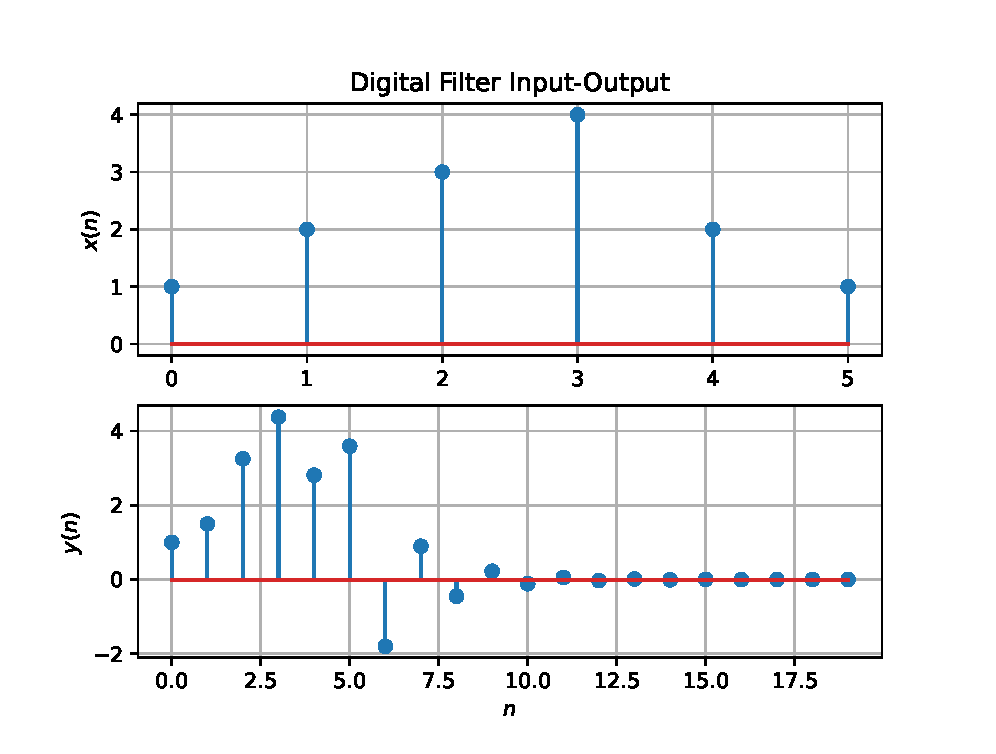
\includegraphics[width=\columnwidth]{./figs/xnyn}
\end{center}
\captionof{figure}{}
\label{fig:xnyn}	
\end{figure}

\item Repeat the above exercise using a C code.
\solution
\begin{lstlisting}
wget https://github.com/Sigma1084/EE3900/raw/master/filer/code/Ex3_xnyn.c
\end{lstlisting}

\end{enumerate}

\section{$Z$-transform}
\begin{enumerate}[label=\thesection.\arabic*]
\item The $Z$-transform of $x(n)$ is defined as
%
\begin{equation}
\label{eq:z_trans}
X(z)={\mathcal {Z}}\{x(n)\}=\sum _{n=-\infty }^{\infty }x(n)z^{-n}
\end{equation}
%
Show that
\begin{equation}
\label{eq:shift1}
{\mathcal {Z}}\{x(n-1)\} = z^{-1}X(z)
\end{equation}
and find
\begin{equation}
	{\mathcal {Z}}\{x(n-k)\} 
\end{equation}
\solution From \eqref{eq:z_trans},
\begin{align}
{\mathcal {Z}}\{x(n-1)\} &=\sum _{n=-\infty }^{\infty }x(n-1)z^{-n}
\\
&=\sum _{n=-\infty }^{\infty }x(n)z^{-n-1} = z^{-1}\sum _{n=-\infty }^{\infty }x(n)z^{-n}
\end{align}
resulting in \eqref{eq:shift1}. Similarly, it can be shown that
%
\begin{equation}
\label{eq:z_trans_shift}
	{\mathcal {Z}}\{x(n-k)\} = z^{-k}X(z)
\end{equation}

\item Obtain $X(z)$ for $x(n)$ defined in problem 
	\ref{def:xn}.
\solution
\begin{equation}
    X(z) =\sum _{n=-\infty }^{\infty }x(n)z^{-n}
\end{equation}
Here, we have $x(n) = 0 \ \forall \ n<0$ and $n\geq6$
\begin{align}
    & X(z) =\sum _{n=0 }^5x(n)z^{-n} \\
    \implies & X(z) = 1 + \frac{2}{z} + \frac{3}{z^2} + \frac{4}{z^3} + \frac{2}{z^4} + \frac{1}{z^5} 
\end{align}

\item Find
%
\begin{equation}
H(z) = \frac{Y(z)}{X(z)}
\end{equation}
%
from  \eqref{eq:iir_filter} assuming that the $Z$-transform is a linear operation.
\\
\solution  Applying \eqref{eq:z_trans_shift} in \eqref{eq:iir_filter},
\begin{align}
Y(z) + \frac{1}{2}z^{-1}Y(z) &= X(z)+z^{-2}X(z)
\\
\implies \frac{Y(z)}{X(z)} &= \frac{1 + z^{-2}}{1 + \frac{1}{2}z^{-1}}
\label{eq:freq_resp}
\end{align}

%
\item Find the Z transform of 
\begin{equation}
\delta(n)
=
\begin{cases}
1 & n = 0
\\
0 & \text{otherwise}
\end{cases}
\end{equation}
and show that the $Z$-transform of
\begin{equation}
\label{eq:unit_step}
u(n)
=
\begin{cases}
1 & n \ge 0
\\
0 & \text{otherwise}
\end{cases}
\end{equation}
is
\begin{equation}
U(z) = \frac{1}{1-z^{-1}}, \quad \abs{z} > 1
\end{equation}
\solution It is easy to show that
\begin{equation}
\delta(n) \ztrans 1
\end{equation}
and from \eqref{eq:unit_step},
\begin{align}
\label{eq:4.14}
U(z) &= \sum _{n= 0}^{\infty}z^{-n}
\\
&=\frac{1}{1-z^{-1}}, \quad \abs{z} > 1
\end{align}
using the formula for the sum of an infinite geometric progression.
%
\item Show that 
\begin{equation}
\label{eq:anun}
a^nu(n) \ztrans \frac{1}{1-az^{-1}} \quad \abs{z} > \abs{a}
\end{equation}
%

\solution 
\begin{equation}
\text{Let } u_a(n) := a^nu(n) =
\begin{cases}
a^n & n \ge 0
\\
0 & \text{otherwise}
\end{cases}
\end{equation}

\begin{align}
\implies U_a(z) & = \sum _{n= 0}^{\infty}z^{-n} . \ a^n
\\
&=\frac{1}{1-az^{-1}}, \quad \abs{z} > \abs{a}
\end{align}
using the formula for the sum of infinite geometric progression with r = $az^{-1}$ and works since $\abs{r} < 1$
%

\item 
Let
\begin{equation}
H\brak{e^{\j \omega}} = H\brak{z = e^{\j \omega}}.
\end{equation}
Plot $\abs{H\brak{e^{\j \omega}}}$.  Comment.  $H(e^{\j \omega})$ is
known as the {\em Discret Time Fourier Transform} (DTFT) of $x(n)$.
\\
\solution The following code plots Fig. \ref{fig:dtft}.
\begin{lstlisting}
wget https://raw.githubusercontent.com/Sigma1084/EE3900/master/filter/code/Ex4_dtft.py
\end{lstlisting}
\begin{align*}
	\left|H\brak{e^{\j\omega}}\right| &= \left|\frac{1 + e^{-2\j\omega}}{1 + \frac{1}{2}e^{-\j\omega}}\right| \\
									  &= \sqrt{\frac{\brak{1 + \cos{2\omega}}^2 + \brak{\sin{2\omega}}^2}{\brak{1 + \frac{1}{2}\cos{\omega}}^2 + \brak{\frac{1}{2}\sin{\omega}}^2}}\\
									  &= \sqrt{\frac{2\brak{1 + \cos{2\omega}}}{\frac{5}{4} + \cos{\omega}}} \\
									  &= \sqrt{\frac{2\brak{2\cos^2{\omega}}}{\frac{5}{4} + \cos{\omega}}} \\
									  &= \frac{4|\cos{\omega}|}{\sqrt{5 + 4\cos{\omega}}}
\end{align*}
Fundamental Period is clearly 2$\pi$.

\begin{figure}[!ht]
\centering
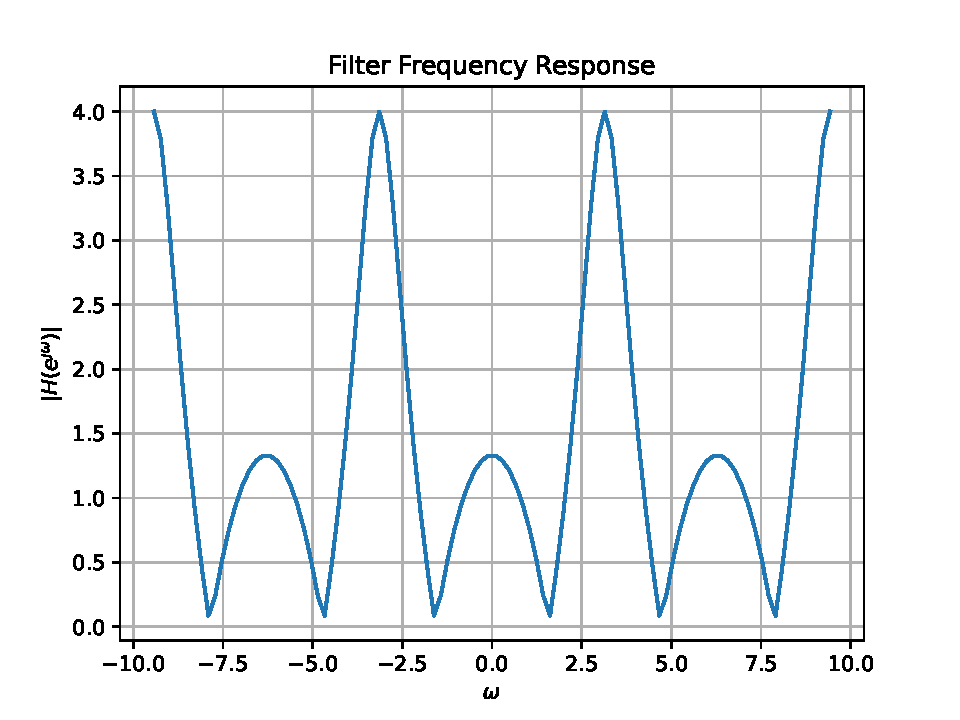
\includegraphics[width=\columnwidth]{./figs/dtft}
\caption{$\abs{H\brak{e^{\j\omega}}}$}
\label{fig:dtft}
\end{figure}

\item Express $h(n)$ in terms of $H\brak{e^{\j \omega}}$.

\[
	H(e^{\j\omega}) &= \sum_{k = -\infty}^{\infty}h(k)e^{-\j\omega k}
\]

We know that,
\begin{align*}
	\int_{-\pi}^{\pi}e^{\j\omega(n - m)}d\omega =
	\begin{cases}
		2\pi & n = m \\
		0 & \textrm{otherwise}
	\end{cases}
\end{align*}

Consider the Inverse Discrete Fourier Transform

\begin{align*}
	&\frac{1}{2\pi}\int_{-\pi}^{\pi}H(e^{\j\omega})e^{j\omega n}d\omega \\
	&= \frac{1}{2\pi}\int_{-\pi}^{\pi}\sum_{m = -\infty}^{\infty}h(m)e^{\j\omega(n - m)}d\omega \\
	&= \frac{1}{2\pi}\sum_{m = -\infty}^{\infty}\int_{-\pi}^{\pi}h(m)e^{\j\omega(n - m)}d\omega \\
	&= \frac{1}{2\pi}2\pi h(n) = h(n)
\end{align*}

Thus, 
\begin{align}
    h(n) &= \frac{1}{2\pi}\int_{-\pi}^{\pi}H(e^{\j\omega})e^{\j\omega n}d\omega
    \label{eq:idtft}
\end{align}

Using \eqref{eq:idtft}, 

\begin{align*}
	h(n) &= \frac{1}{2\pi}\int_{-\pi}^{\pi}\frac{1 + e^{-2\j\omega}}{1 + \frac{1}{2}e^{-\j\omega}}e^{\j\omega n}d\omega
	\label{eq:idtft}
\end{align*}

This is solved and expressed as a function of n in 5.1

\end{enumerate}


\section{Impulse Response}

\begin{enumerate}[label=\thesection.\arabic*]

\item Using long division, compute $h(n)$ for $n < 5$ from $H(z)$.

\solution We substitute $x := z^{-1}$, and perform the long division.

\polylongdiv{1 + x^2}{1 + \frac{1}{2}x}

Thus,
\begin{align}
	H(z) &= -4 + 2z^{-1} + \frac{5}{1 + \frac{1}{2}z^{-1}} \\
		 &= -4 + 2z^{-1} + 5\sum_{n = 0}^{\infty}\brak{-\frac{1}{2}}^nz^{-n} \\
		 &= 1 - \frac{1}{2}z^{-1} + 5\sum_{n = 2}^{\infty}\brak{-\frac{1}{2}}^nz^{-n} \\
		 &= \sum_{n = 0}^{\infty}\brak{-\frac{1}{2}}^nz^{-n} + 4\sum_{n = 2}^{\infty}\brak{-\frac{1}{2}}^nz^{-n} \\
		 &= \sum_{n = -\infty}^{\infty}u(n)\brak{-\frac{1}{2}}^nz^{-n} + \nonumber \\
		 &\sum_{n = -\infty}^{\infty}u(n - 2)\brak{-\frac{1}{2}}^{n - 2}z^{-n}
\end{align}

Therefore, from \eqref{eq:z_trans}, 
\begin{align}
	h(n) = \brak{-\frac{1}{2}}^{n}u(n) + \brak{-\frac{1}{2}}^{n-2}u(n-2)
\end{align}


\item \label{prob:impulse_resp}
Find an expression for $h(n)$ using $H(z)$, given that 
%in Problem \ref{eq:ztransab} and \eqref{eq:anun}, given that
\begin{equation}
\label{eq:impulse_resp}
h(n) \ztrans H(z)
\end{equation}
and there is a one to one relationship between $h(n)$ and $H(z)$. $h(n)$ is known as the {\em impulse response} of the
system defined by \eqref{eq:iir_filter}.
\\
\solution From \eqref{eq:freq_resp},
\begin{align}
H(z) &= \frac{1}{1 + \frac{1}{2}z^{-1}} + \frac{ z^{-2}}{1 + \frac{1}{2}z^{-1}}
\\
\implies h(n) &= \brak{-\frac{1}{2}}^{n}u(n) + \brak{-\frac{1}{2}}^{n-2}u(n-2)
\end{align}
using \eqref{eq:anun} and \eqref{eq:z_trans_shift}.
\item Sketch $h(n)$. Is it bounded?
\\
\solution The following code plots Fig. \ref{fig:hn}.
\begin{lstlisting}
wget https://raw.githubusercontent.com/Sigma1084/EE3900/master/filter/code/Ex5_hn.py
\end{lstlisting}
\begin{figure}[!ht]
\centering
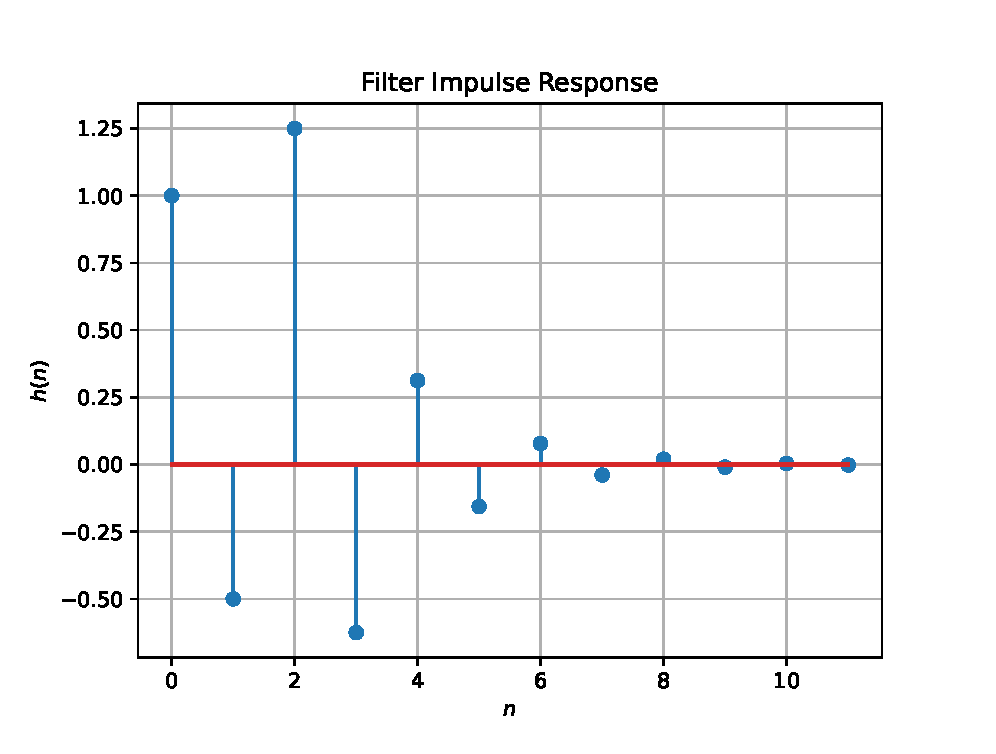
\includegraphics[width=\columnwidth]{./figs/hn}
\caption{$h(n)$ as the inverse of $H(z)$}
\label{fig:hn}
\end{figure}

We see that $h(n)$ is bounded. For large $n$,
\begin{align*}
	h(n) &= \brak{-\frac{1}{2}}^n + \brak{-\frac{1}{2}}^{n - 2} \\
		 &= \brak{-\frac{1}{2}}^{n}\brak{4 + 1} = 5\brak{-\frac{1}{2}}^n
\end{align*}

\item Convergent? Justify using ratio test. \\
\solution

$\lim_{n \to \infty}\left|\frac{h(n + 1)}{h(n)}\right| = \frac{1}{2} < 1$ Therefore, $h(n)$ converges.

%
\item The system with $h(n)$ is defined to be stable if
\begin{equation}
\sum_{n=-\infty}^{\infty}h(n) < \infty
\end{equation}
Is the system defined by \eqref{eq:iir_filter} stable for the impulse response in \eqref{eq:impulse_resp}?

\solution
\begin{align*}
	\sum_{n = -\infty}^{\infty}h\brak{n} &= \sum_{n = -\infty}^{\infty}
	\brak{-\frac{1}{2}}^nu\brak{n} + \brak{-\frac{1}{2}}^{n - 2}u\brak{n - 2} \\
	&= 2\brak{\frac{1}{1 + \frac{1}{2}}} = \frac{4}{3} < \infty
\end{align*}
Thus, the given system is stable.

%

\item Verify the above result using a python code.

\solution
The below code calculates around 100000 terms of $h(n)$ for an approximate since we know $h(n)$ is convergent

\begin{lstlisting}
wget https://raw.githubusercontent.com/Sigma1084/EE3900/master/filter/code/Ex5_verify_hn.py
\end{lstlisting}

%
\item 
Compute and sketch $h(n)$ using 
\begin{equation}
\label{eq:iir_filter_h}
h(n) + \frac{1}{2}h(n-1) = \delta(n) + \delta(n-2), 
\end{equation}
%
This is the definition of $h(n)$.
\\
\solution The following code plots Fig. \ref{fig:hndef}. Note that this is the same as Fig. 
\ref{fig:hn}. 
%
\begin{lstlisting}
wget https://raw.githubusercontent.com/Sigma1084/EE3900/master/filter/code/Ex5_hndef.py
\end{lstlisting}
\begin{figure}[!ht]
\centering
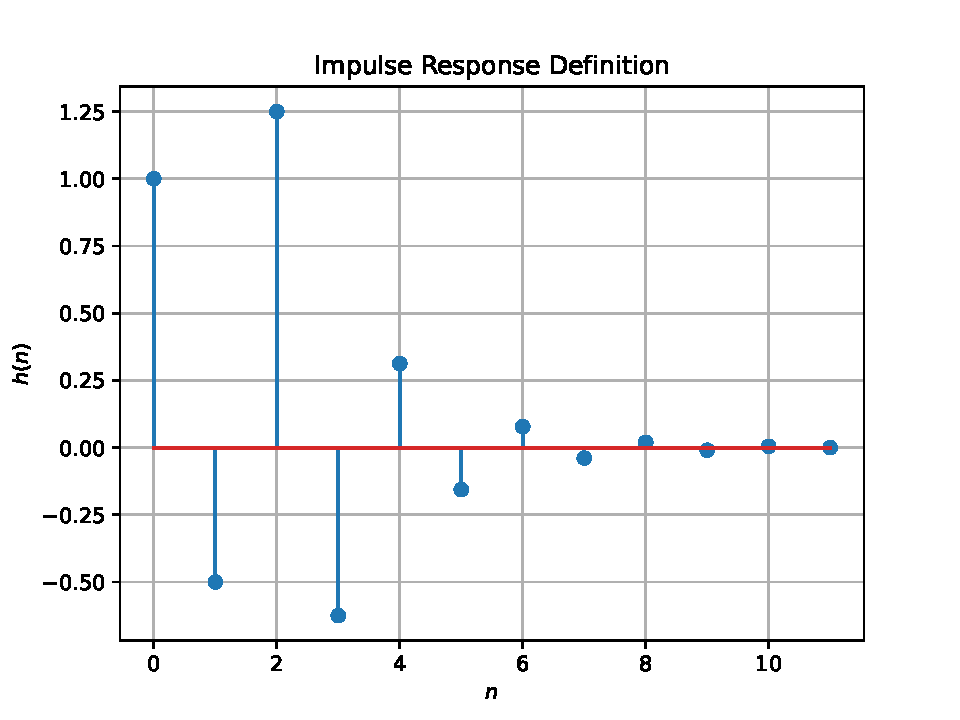
\includegraphics[width=\columnwidth]{./figs/hndef}
\caption{$h(n)$ from the definition}
\label{fig:hndef}
\end{figure}
%

\item Compute 
%
\begin{equation}
\label{eq:convolution}
y(n) = x(n)*h(n) = \sum_{k=-\infty}^{\infty}x(k)h(n-k)
\end{equation}
%
Comment. The operation in \eqref{eq:convolution} is known as
{\em convolution}.
%
\\
\solution The following code plots Fig. \ref{fig:ynconv}. Note that this is the same as 
$y(n)$ in  Fig. 
\ref{fig:xnyn}. 
%
\begin{lstlisting}
wget https://raw.githubusercontent.com/Sigma1084/EE3900/master/filter/code/Ex5_ynconv.py
\end{lstlisting}
\begin{figure}[!ht]
\centering
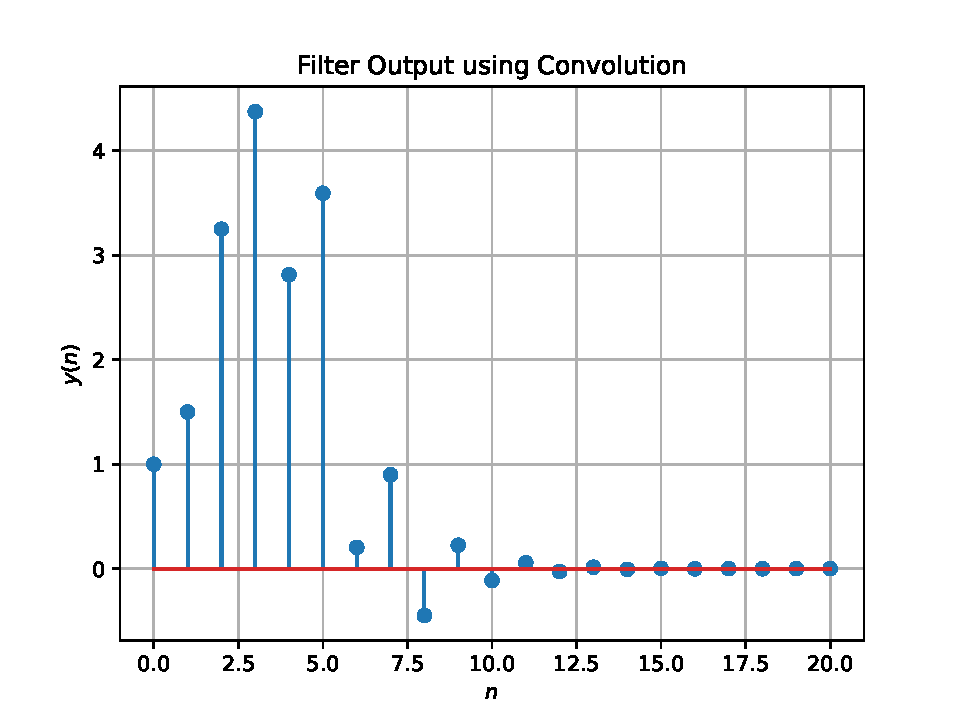
\includegraphics[width=\columnwidth]{./figs/ynconv}
\caption{$y(n)$ from the definition of convolution}
\label{fig:ynconv}
\end{figure}

%

\item Express the above convolution using a Teoplitz matrix. \\

\solution
\begin{align*}
	\mtx{y} &= \mtx{x} \circledast \mtx{h}\\
	\mtx{y} &= 
	\begin{pmatrix}
		h_1 & 0 & . & . & . & 0 \\
		h_2 & h_1 & . & . & . & 0 \\
		h_3 & h_2 & h_1 & . & . & 0 \\
		. & . & . & . & . & . \\
		0 & . & . & h_3 & h_2 & h_1 \\
		0 & . & . & . & h_2 & h_1 \\
		0 & . & . & . & 0 & h_1
	\end{pmatrix}
	\begin{pmatrix}
		x_1 \\ x_2 \\ \vdots \\ x_n
	\end{pmatrix}
\end{align*}

%

\item Show that
\begin{equation}
\label{eq:yn}
y(n) =  \sum_{k=-\infty}^{\infty}x(n-k)h(k)
\end{equation}
\end{enumerate}

\solution Substituting k = n - k in \eqref{eq:yn}, we get
\begin{equation}
y(n) =  \sum_{n-k=-\infty}^{\infty}x(k)h(n-k)
\end{equation}
This is clearly equivalent to \eqref{eq:convolution}

%

\section{DFT}

\begin{enumerate}[label=\thesection.\arabic*]

\item
Compute
\begin{equation}
X(k) \define \sum _{n=0}^{N-1}x(n) e^{-\j2\pi kn/N}, \quad k = 0,1,\dots, N-1
\end{equation}
and $H(k)$ using $h(n)$.

\solution
The following code yields X(k) and H(k)
\begin{lstlisting}
wget https://raw.githubusercontent.com/Sigma1084/EE3900/master/filter/code/Ex6_XkHk.py
\end{lstlisting}

\item Compute 
\begin{equation}
Y(k) = X(k)H(k)
\end{equation}

\solution
The following code yields Yk
\begin{lstlisting}
wget https://raw.githubusercontent.com/Sigma1084/EE3900/master/filter/code/Ex6_Yk.py
\end{lstlisting}


\item Compute
\begin{equation}
 y\brak{n}={\frac {1}{N}}\sum _{k=0}^{N-1}Y\brak{k}\cdot e^{\j 2\pi kn/N},\quad n = 0,1,\dots, N-1
 \label{eq:inv-ft}
\end{equation}

\\
\solution The following code plots Fig. \ref{fig:ynconv}. Note that this is the same as 
$y(n)$ in  Fig. 
\ref{fig:xnyn}. 
%
\begin{lstlisting}
wget https://raw.githubusercontent.com/Sigma1084/EE3900/master/filter/code/Ex6_yndft.py
\end{lstlisting}

\begin{figure}[!ht]
    \centering
    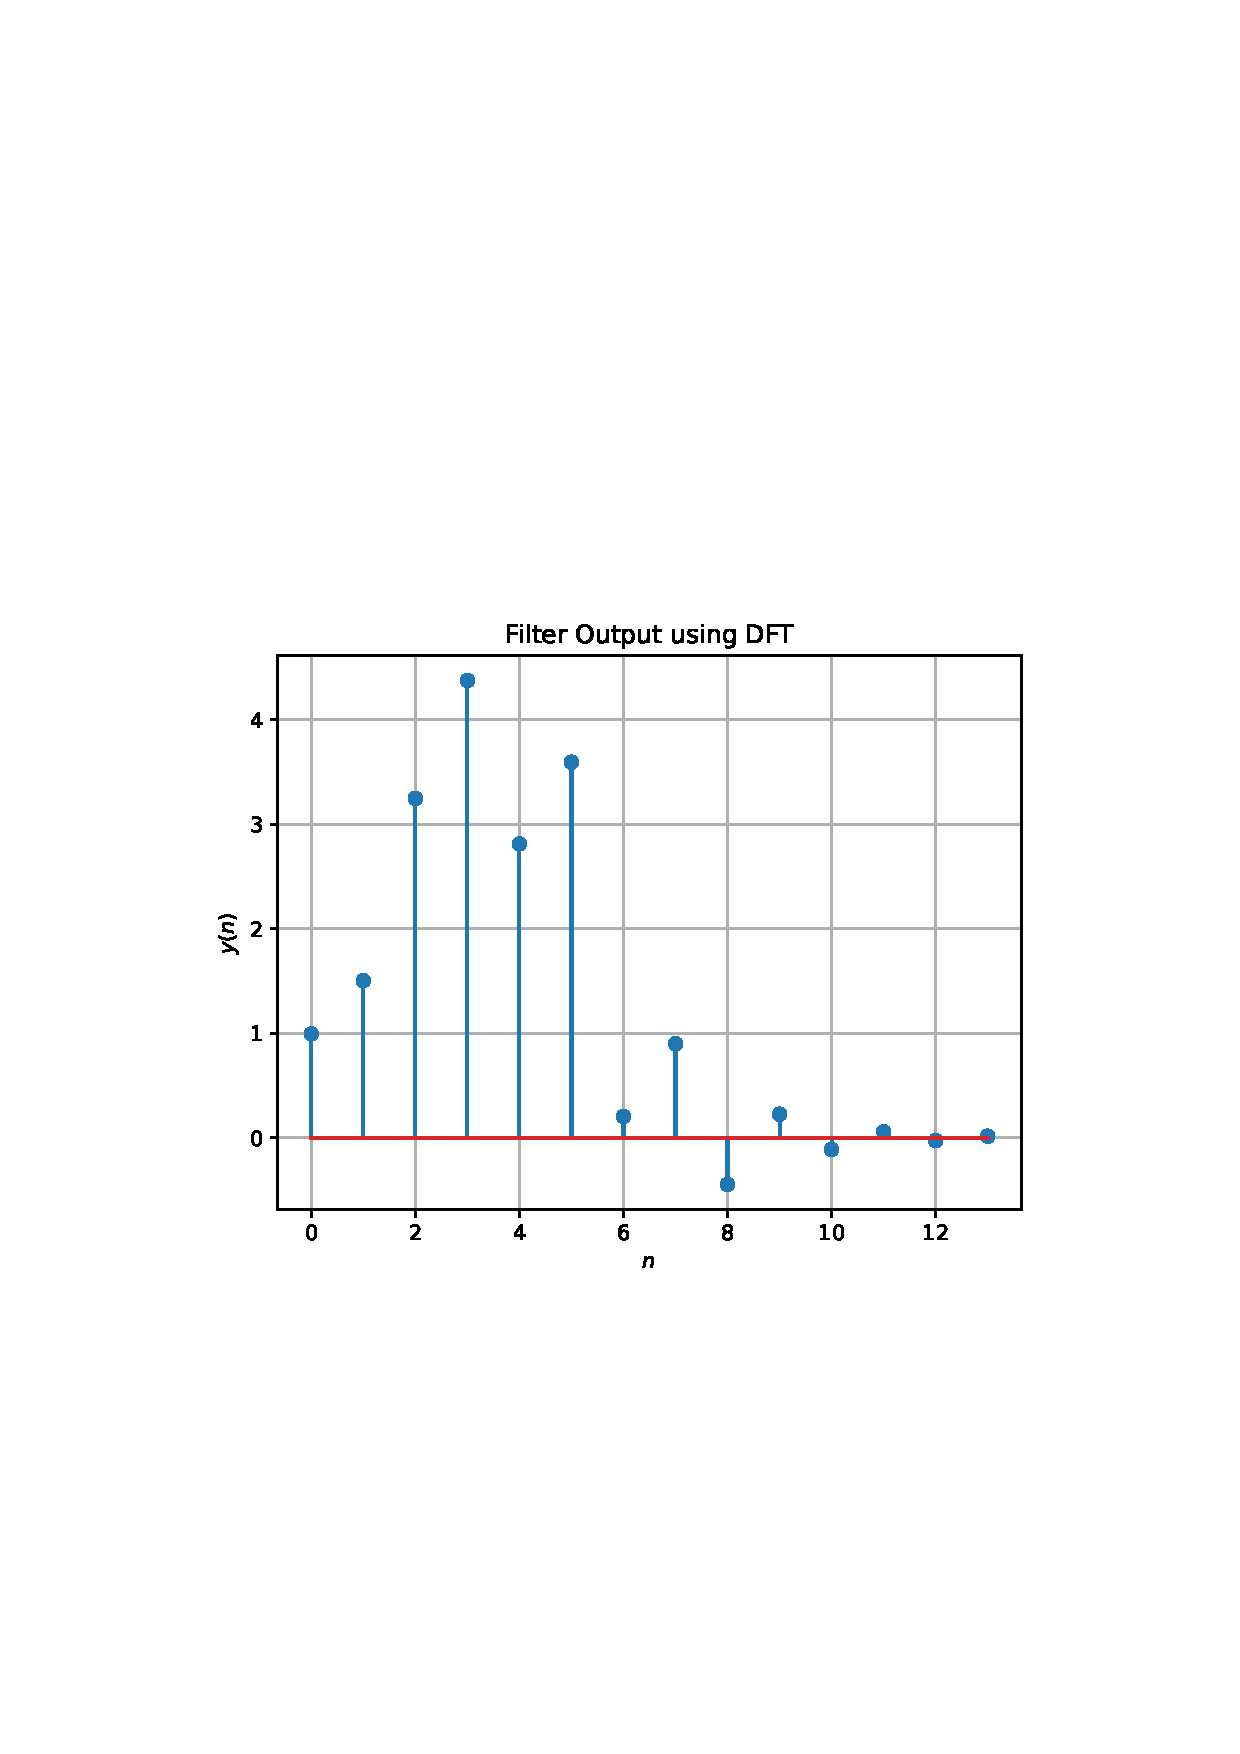
\includegraphics[width=\columnwidth]{./figs/yndft}
    \caption{$y(n)$ from the DFT}
    \label{fig:yndft}
\end{figure}

\item Repeat the previous exercise by computing $X(k), H(k)$ and $y(n)$ through FFT and  IFFT.

\solution The following code plots Fig. \ref{fig:ynfft}. Note that this is the same as $y(n)$ in Fig. \ref{fig:xnyn}

\begin{lstlisting}
$ wget https://raw.githubusercontent.com/Sigma1084/EE3900/master/filter/code/Ex6_ynfft.py
\end{lstlisting}

\begin{figure}
	\centering
	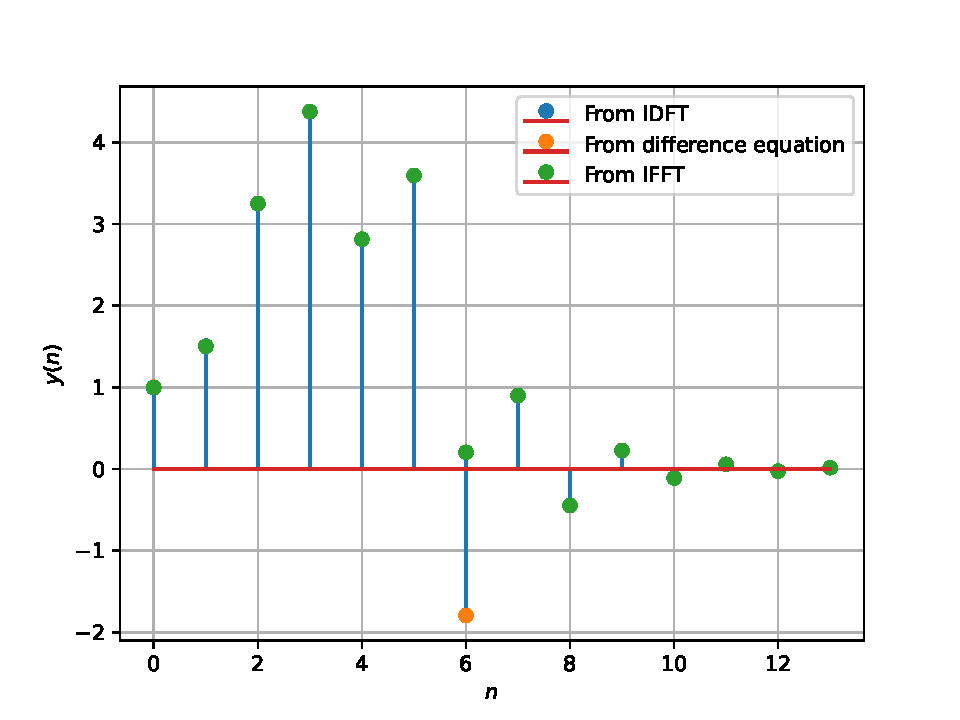
\includegraphics[width=\columnwidth]{figs/ynfft.pdf}
	\caption{$y(n)$ using FFT and IFFT}
	\label{fig:ynfft}
\end{figure}


\end{enumerate}
%


\pagebreak

\section{FFT}

\begin{enumerate}[label=\thesection.\arabic*]
\numberwithin{equation}{section}
    \item The DFT of $x(n)$ is given by
    \begin{align}
        X(k) \triangleq \sum_{n=0}^{N-1} x(n) e^{-j 2 \pi k n / N}, \quad k=0,1, \ldots, N-1
    \end{align}
\item Let 
	\begin{align}
W_{N} = e^{-j2\pi/N} 
	\end{align}
		Then the $N$-point {\em DFT matrix} is defined as 
	\begin{align}
		\vec{F}_{N} = \sbrak{W_{N}^{mn}}, \quad 0 \le m,n \le N-1 
	\end{align}
	where $W_{N}^{mn}$ are the elements of $\vec{F}_{N}$.
\item Let 
	\begin{align}
		\vec{I}_4 = \myvec{\vec{e}_4^{1} &\vec{e}_4^{2} &\vec{e}_4^{3} &\vec{e}_4^{4} }
	\end{align}
		be the $4\times 4$ identity matrix.  Then the 4 point {\em DFT permutation matrix} is defined as 
	\begin{align}
		\vec{P}_4 = \myvec{\vec{e}_4^{1} &\vec{e}_4^{3} &\vec{e}_4^{2} &\vec{e}_4^{4} }
	\end{align}
\item The 4 point {\em DFT diagonal matrix} is defined as 
	\begin{align}
		\vec{D}_4 = diag\myvec{W_{8}^{0} & W_{8}^{1} & W_{8}^{2} & W_{8}^{3}}
	\end{align}

\item Show that 
\begin{equation}
    W_{N}^{2}=W_{N/2}
\end{equation}

\solution
\begin{align}
	W_N^2 = \brak{e^{-\frac{\text{j}2\pi}{N}}}^2 = e^{-\frac{\text{j}2\pi}{N/2}} = W_{N/2}
	\label{eq:n-2}
\end{align}

%    \item Find $\vec{P}_6$.
%    \item Find $\vec{D}_3$.

\item Show that 
\begin{equation}
	\vec{F}_{4}=
\begin{bmatrix}
	\vec{I}_{2} & \vec{D}_{2} \\
\vec{I}_{2} & -\vec{D}_{2}
\end{bmatrix}
\begin{bmatrix}
\vec{F}_{2} & 0 \\
0 & \vec{F}_{2}
\end{bmatrix}
\vec{P}_{4}
\end{equation}

\solution
\begin{align}
	&\mymat{\vec{I}_2 & \vec{D}_2 \\ \vec{I}_2 & -\vec{D}_2} \mymat{\vec{F}_2 & 0 \\ 0 & \vec{F}_2} \\
	= &\mymat{\vec{F}_2 & \vec{D}_2\vec{F}_2 \\ \vec{F}_2 & -\vec{D}_2\vec{F}_2} \\
	= &\mymat{\myvec{1&1\\1&-1} & \myvec{1&0\\0&-j}\myvec{1&1\\1&-1} \\ \myvec{1&1\\1&-1} & -\myvec{1&0\\0&-j}\myvec{1&1\\1&-1}}\\
	= &\mymat{1&1&1&1 \\ 1&-1&-j&j \\ 1&1&-1&-1 \\ 1&-1&j&-j}\\
	&\vec{P}_4 = \mymat{1&0&0&0 \\ 0&0&1&0 \\ 0&1&0&0 \\ 0&0&0&1}
\end{align}

\begin{align}
	&\mymat{1&1&1&1 \\ 1&-1&-j&j \\ 1&1&-1&-1 \\ 1&-1&j&-j} \mymat{1&0&0&0 \\ 0&0&1&0 \\ 0&1&0&0 \\ 0&0&0&1}\\
	&= \mymat{1 & 1 & 1 & 1 \\ 1 & -\text{\j} & -1 & \text{\j} \\ 1 & -1 & 1 & -1 \\ 1 & \text{\j} & -1 & -\text{\j}} \\
	&= \mymat{W_4^0 & W_4^0 & W_4^0 & W_4^0 \\ W_4^0 & W_4^1 & W_4^2 & W_4^3 \\ W_4^0 & W_4^2 & W_4^4 & W_4^6 \\ W_4^0 & W_4^3 & W_4^6 & W_4^9} \\
	&= \vec{F}_4
\end{align}

%

\item Show that 
\begin{equation}
\vec{F}_{N}=
\begin{bmatrix}
\vec{I}_{N/2} & \vec{D}_{N/2} \\
\vec{I}_{N/2} & -\vec{D}_{N/2}
\end{bmatrix}
\begin{bmatrix}
\vec{F}_{N/2} & 0 \\
0 & \vec{F}_{N/2}
\end{bmatrix}
\vec{P}_{N}
\end{equation}

\solution Observe that for even $N$ and letting $\vec{f}_N^i$ denote the $i^{\text{th}}$ column of $\vec{F}_N$,
\begin{align}
	\myvec{\vec{D}_{N/2}\vec{F}_{N/2} \\ -\vec{D}_{N/2}\vec{F}_{N/2}} = \myvec{\vec{f}_N^{2} & \vec{f}_N^{4} & \ldots & \vec{f}_N^{N}}
\end{align}
and
\begin{align}
	\myvec{\vec{I}_{N/2}\vec{F}_{N/2} \\ \vec{I}_{N/2}\vec{F}_{N/2}} = \myvec{\vec{f}_N^{1} & \vec{f}_N^{3} & \ldots & \vec{f}_N^{N - 1}}
\end{align}

Thus,
\begin{align}
	&\myvec{\vec{I}_2\vec{F}_2 & \vec{D}_2\vec{F}_2 \\ \vec{I}_2\vec{F}_2 & -\vec{D}_2\vec{F}_2} = \myvec{\vec{I}_{N/2} & \vec{D}_{N/2} \\ \vec{I}_{N/2} & -\vec{D}_{N/2}}\myvec{\vec{F}_{N/2} & 0 \\ 0 & \vec{F}_{N/2}} \notag \\
	&= \myvec{\vec{f}_N^{1} & \ldots & \vec{f}_N^{N - 1} & \vec{f}_N^{2} & \ldots & \vec{f}_N^{N}}
\end{align}
and so,

\begin{align}
	&\myvec{\vec{I}_{N/2} & \vec{D}_{N/2} \\ \vec{I}_{N/2} & -\vec{D}_{N/2}}\myvec{\vec{F}_{N/2} & 0 \\ 0 & \vec{F}_{N/2}}\vec{P}_{N} \notag \\
	&= \myvec{\vec{f}_N^{1} & \vec{f}_N^{2} & \ldots & \vec{f}_N^{N}} = \vec{F}_N
\end{align}

%

\item Find
    \begin{align}
	     \vec{P}_4 \vec{x}
    \end{align}

\solution
\begin{align}
	\vec{P}_4\vec{x} = \myvec{\vec{e}_4^1 & \vec{e}_4^3 & \vec{e}_4^2 & \vec{e}_4^4}\myvec{x(0)\\x(1)\\x(2)\\x(3)} = \myvec{x(0)\\x(2)\\x(1)\\x(3)}
	\label{eq:x-permute}
\end{align}

%

\item Show that 
    \begin{align}
	    \vec{X} = \vec{F}_N \vec{x}
	    \label{eq:dft-mat-def}
    \end{align}
		where $\vec{x}, \vec{X}$ are the vector representations of $x(n), X(k)$ respectively.

\solution Writing the terms of $X$, 
\begin{align}
	X(0) &= x(0) + x(1) + \ldots + x(N - 1) \\
	X(1) &= x(0) + x(1)e^{-\frac{\text{j}2\pi}{N}} + \ldots + \nonumber \\
		 &+ x(N - 1)e^{-\frac{\text{j}2(N - 1)\pi}{N}} \\
		 &\vdots \nonumber \\
	X(N - 1) &= x(0) + x(1)e^{-\frac{\text{j}2(N - 1)\pi}{N}} + \ldots + \nonumber \\
			 &+ x(N - 1)e^{-\frac{\text{j}2(N - 1)(N - 1)\pi}{N}}	
\end{align}
Clearly, the term in the $m^{\text{th}}$ row and $n^{\text{th}}$ column is given by ($0 \leq m \leq N - 1$ and $0 \leq n \leq N - 1$) 
\begin{align}
	T_{mn} & = ( x(n) e^{-\frac{\text{j}2n\pi}{N}} ) e^{-\frac{\text{j}2m\pi}{N}} \\
	& = x(n) e^{-\frac{\text{j}2mn\pi}{N}}
\end{align}

\begin{align}
	\implies \vec{X} = \vec{F}_N\vec{x}
\end{align}

%





%

\item Derive the following Step-by-step visualisation  of
8-point FFTs into 4-point FFTs and so on
\begin{equation}
\begin{bmatrix}
X(0) \\ 
X(1) \\ 
X(2) \\ 
X(3)
\end{bmatrix}
=
\begin{bmatrix}
X_{1}(0) \\ 
X_{1}(1)\\ 
X_{1}(2)\\
X_{1}(3)\\
\end{bmatrix}
+
\begin{bmatrix}
W^{0}_{8} & 0 & 0 & 0\\
0 & W^{1}_{8} & 0 & 0\\
0 & 0 & W^{2}_{8} & 0\\
0 & 0 & 0 & W^{3}_{8}
\end{bmatrix}
\begin{bmatrix}
X_{2}(0) \\ 
X_{2}(1) \\ 
X_{2}(2) \\
X_{2}(3)
\end{bmatrix}
\end{equation}
\begin{equation}
\begin{bmatrix}
X(4) \\ 
X(5) \\ 
X(6) \\ 
X(7)
\end{bmatrix}
=
\begin{bmatrix}
X_{1}(0) \\ 
X_{1}(1)\\ 
X_{1}(2)\\
X_{1}(3)\\
\end{bmatrix}
-
\begin{bmatrix}
W^{0}_{8} & 0 & 0 & 0\\
0 & W^{1}_{8} & 0 & 0\\
0 & 0 & W^{2}_{8} & 0\\
0 & 0 & 0 & W^{3}_{8}
\end{bmatrix}
\begin{bmatrix}
X_{2}(0) \\ 
X_{2}(1) \\ 
X_{2}(2) \\
X_{2}(3)
\end{bmatrix}
\end{equation}
4-point FFTs into 2-point FFTs
\begin{equation}
\begin{bmatrix}
X_{1}(0) \\ 
X_{1}(1)\\ 
\end{bmatrix}
=
\begin{bmatrix}
X_{3}(0) \\ 
X_{3}(1)\\ 
\end{bmatrix}
+
\begin{bmatrix}
W^{0}_{4} & 0\\
0 & W^{1}_{4}
\end{bmatrix}
\begin{bmatrix}
X_{4}(0) \\ 
X_{4}(1) \\ 
\end{bmatrix}
\end{equation}
\begin{equation}
\begin{bmatrix}
X_{1}(2) \\ 
X_{1}(3)\\ 
\end{bmatrix}
=
\begin{bmatrix}
X_{3}(0) \\ 
X_{3}(1)\\ 
\end{bmatrix}
-
\begin{bmatrix}
W^{0}_{4} & 0\\
0 & W^{1}_{4}
\end{bmatrix}
\begin{bmatrix}
X_{4}(0) \\ 
X_{4}(1) \\ 
\end{bmatrix}
\end{equation}
\begin{equation}
\begin{bmatrix}
X_{2}(0) \\ 
X_{2}(1)\\ 
\end{bmatrix}
=
\begin{bmatrix}
X_{5}(0) \\ 
X_{5}(1)\\ 
\end{bmatrix}
+
\begin{bmatrix}
W^{0}_{4} & 0\\
0 & W^{1}_{4}
\end{bmatrix}
\begin{bmatrix}
X_{6}(0) \\ 
X_{6}(1) \\ 
\end{bmatrix}
\end{equation}
\begin{equation}
\begin{bmatrix}
X_{2}(2) \\ 
X_{2}(3)\\ 
\end{bmatrix}
=
\begin{bmatrix}
X_{5}(0) \\ 
X_{5}(1)\\ 
\end{bmatrix}
-
\begin{bmatrix}
W^{0}_{4} & 0\\
0 & W^{1}_{4}
\end{bmatrix}
\begin{bmatrix}
X_{6}(0) \\ 
X_{6}(1) \\ 
\end{bmatrix}
\end{equation}
\begin{equation}
P_{8}
\begin{bmatrix}
x(0) \\ 
x(1) \\ 
x(2) \\ 
x(3) \\ 
x(4) \\ 
x(5) \\
x(6) \\
x(7)
\end{bmatrix}
 = 
\begin{bmatrix}
x(0) \\ 
x(2) \\ 
x(4) \\ 
x(6) \\
x(1) \\ 
x(3) \\ 
x(5) \\
x(7)
\end{bmatrix}
\end{equation}
\begin{equation}
P_{4}
\begin{bmatrix}
x(0) \\ 
x(2) \\ 
x(4) \\ 
x(6) \\
\end{bmatrix}
 = 
\begin{bmatrix}
x(0) \\ 
x(4) \\ 
x(2) \\
x(6)
\end{bmatrix}
\end{equation}
\begin{equation}
P_{4}
\begin{bmatrix}
x(1) \\ 
x(3) \\ 
x(5) \\
x(7)
\end{bmatrix}
 = 
\begin{bmatrix}
x(1) \\ 
x(5) \\ 
x(3) \\ 
x(7) \\
\end{bmatrix}
\end{equation}
Therefore,
\begin{equation}
\begin{bmatrix}
X_{3}(0) \\ 
X_{3}(1)\\ 
\end{bmatrix}
= F_{2}
\begin{bmatrix}
x(0) \\ 
x(4) \\ 
\end{bmatrix}
\end{equation}
\begin{equation}
\begin{bmatrix}
X_{4}(0) \\ 
X_{4}(1)\\ 
\end{bmatrix}
= F_{2}
\begin{bmatrix}
x(2) \\ 
x(6) \\ 
\end{bmatrix}
\end{equation}
\begin{equation}
\begin{bmatrix}
X_{5}(0) \\ 
X_{5}(1)\\ 
\end{bmatrix}
= F_{2}
\begin{bmatrix}
x(1) \\ 
x(5) \\ 
\end{bmatrix}
\end{equation}
\begin{equation}
\begin{bmatrix}
X_{6}(0) \\ 
X_{6}(1)\\ 
\end{bmatrix}
= F_{2}
\begin{bmatrix}
x(3) \\ 
x(7) \\ 
\end{bmatrix}
\end{equation}

%


\solution We write out the values of performing an 8-point FFT on $\vec{x}$ as follows.
\begin{align}
	X(k) &= \sum_{n = 0}^{7}x(n)e^{-\frac{\j2kn\pi}{8}} \\
		 &= \sum_{n = 0}^{3}\brak{x(2n)e^{-\frac{\j2kn\pi}{4}} + e^{-\frac{\j2k\pi}{8}}x(2n + 1)e^{-\frac{\j2kn\pi}{4}}} \\
		 &= X_1(k) + e^{-\frac{\j2k\pi}{4}}X_2(k) 
\end{align}
where $\vec{X}_1$ is the 4-point FFT of the even-numbered terms and $\vec{X}_2$ is the 4-point FFT of the odd numbered terms. Noticing that for $k \geq 4$,
\begin{align}
	X_1(k) &= X_1(k - 4) \\
	e^{-\frac{\j2k\pi}{8}} &= -e^{-\frac{\j2(k - 4)\pi}{8}}
\end{align}
we can now write out $X(k)$ in matrix form.
\begin{align}
	X_1(k) &= \sum_{n = 0}^{3}x_1(n)e^{-\frac{\j2kn\pi}{8}} \\
		 &= \sum_{n = 0}^{1}\brak{x_1(2n)e^{-\frac{\j2kn\pi}{4}} + e^{-\frac{\j2k\pi}{8}}x_2(2n + 1)e^{-\frac{\j2kn\pi}{4}}} \\
		 &= X_3(k) + e^{-\frac{\j2k\pi}{4}}X_4(k) 
\end{align}
using $x_1(n) = x(2n)$ and $x_2(n) = x(2n + 1)$. Thus we can write the 2-point FFTs
\begin{align}
\begin{bmatrix}
X_{3}(0) \\ 
X_{3}(1)\\ 
\end{bmatrix}
= F_{2}
\begin{bmatrix}
x(0) \\ 
x(4) \\ 
\end{bmatrix} \\
\begin{bmatrix}
X_{4}(0) \\ 
X_{4}(1)\\ 
\end{bmatrix}
= F_{2}
\begin{bmatrix}
x(2) \\ 
x(6) \\ 
\end{bmatrix}
\end{align}
Using a similar idea for the terms $X_2$, 
\begin{align}
\begin{bmatrix}
X_{5}(0) \\ 
X_{5}(1)\\ 
\end{bmatrix}
= F_{2}
\begin{bmatrix}
x(1) \\ 
x(5) \\ 
\end{bmatrix} \\
\begin{bmatrix}
X_{6}(0) \\ 
X_{6}(1)\\ 
\end{bmatrix}
= F_{2}
\begin{bmatrix}
x(3) \\ 
x(7) \\ 
\end{bmatrix}
\end{align}
But observe that from \eqref{eq:x-permute},
\begin{align}
	\vec{P}_8\vec{x} &= \myvec{\vec{x}_1\\\vec{x}_2} \\
	\vec{P}_4\vec{x}_1 &= \myvec{\vec{x}_3\\\vec{x}_4} \\ 
	\vec{P}_4\vec{x}_2 &= \myvec{\vec{x}_5\\\vec{x}_6}
\end{align}
where we define $x_3(k) = x(4k)$, $x_4(k) = x(4k + 2)$, $x_5(k) = x(4k + 1)$, and $x_6(k) = x(4k + 3)$ for $k = 0, 1$.


%

\item For 
    \begin{align}
	    \vec{x} = \myvec{1\\2\\3\\4\\2\\1}
        \label{eq:equation1}
    \end{align}
    compte the DFT using \eqref{eq:dft-mat-def}
	    
\item Repeat the above exercise using the FFT
    after zero padding $\vec{x}$.
    
\solution
The following code yields the DFT Matrix of x
\begin{lstlisting}
$ wget https://raw.githubusercontent.com/Sigma1084/EE3900/main/filter/codes/Ex7_dftmatrix.py
\end{lstlisting}


%

%	    \eqref{eq:fft-mat-def}

%

\item Write a C program to compute the 8-point FFT.

\solution

\begin{lstlisting}
$ wget https://raw.githubusercontent.com/Sigma1084/EE3900/main/filter/codes/Ex7_8point.c
\end{lstlisting}

Run the code using the command below

\begin{lstlisting}
$ gcc Ex7_8point.c -lm -o Ex7.out && ./Ex7.out
\end{lstlisting}

\end{enumerate}



\section{Exercises}
Answer the following questions by looking at the python code in Problem \ref{prob:output}.
\begin{enumerate}[label=\thesection.\arabic*]

\item
The command
\begin{lstlisting}
output_signal = signal.lfilter(b, a, input_signal)
\end{lstlisting}
in Problem \ref{prob:output} is executed through the following difference equation
\begin{equation}
\label{eq:iir_filter_gen}
    \sum _{m=0}^{M}a\brak{m}y\brak{n-m}=\sum _{k=0}^{N}b\brak{k}x\brak{n-k}
\end{equation}
%
where the input signal is $x(n)$ and the output signal is $y(n)$ with initial values all 0. Replace
\textbf{signal.filtfilt} with your own routine and verify.
%

\item Repeat all the exercises in the previous sections for the above $a$ and $b$.

\item What is the sampling frequency of the input signal?

\\
\solution
Sampling frequency(fs)=44.1kHZ.

\item
What is type, order and  cutoff-frequency of the above butterworth filter
\\
\solution
The given butterworth filter is low pass with order=2 and cutoff-frequency=4kHz.
%

\item
Modifying the code with different input parameters and to get the best possible output. \\
% \solution A better filtering was found on setting the order of the filter to be 7

%
\end{enumerate}

\end{document}
